\documentclass[tikz,border=3pt]{standalone}
\usepackage[utf8]{inputenc}
\usepackage[T1]{fontenc}
\usepackage{lmodern}
\renewcommand{\familydefault}{\sfdefault}
\usepackage{sansmath}\sansmath
\usepackage{chemfig}
\usepackage{pgfplots}\pgfplotsset{compat=1.18,/pgf/number format/use comma,/pgf/number format/1000 sep={.}}
\usetikzlibrary{arrows.meta,calc,positioning,decorations.pathmorphing,patterns}
% paleta del sitio
\definecolor{nar}{HTML}{E8680C}\definecolor{narc}{HTML}{FFB35C}\definecolor{hielo}{HTML}{FFF3E8}
\definecolor{tinta}{HTML}{1D1D1F}\definecolor{gris}{HTML}{6E6E73}\definecolor{lila}{HTML}{7C5CF0}
\definecolor{azul}{HTML}{2F6FD6}\definecolor{menta}{HTML}{17A673}\definecolor{coral}{HTML}{E8342A}
\newcommand{\sinapsis}{%
% terminal presinaptico
\draw[nar,line width=1pt,fill=narc!30] (-0.55,5.4) -- (-0.55,4.3) .. controls (-3.1,4.1) and (-3.3,1.6) .. (-2.5,1.3) -- (2.5,1.3) .. controls (3.3,1.6) and (3.1,4.1) .. (0.55,4.3) -- (0.55,5.4);
% neurona postsinaptica
\draw[azul,line width=1pt,fill=azul!10] (-3.4,-1.2) -- (-3.4,0.4) -- (3.4,0.4) -- (3.4,-1.2);
% mitocondria
\draw[nar,fill=narc!60] (1.2,3.55) ellipse (0.5 and 0.22);
\draw[nar] (0.85,3.55) .. controls (0.95,3.7) and (1.05,3.4) .. (1.15,3.55) .. controls (1.25,3.7) and (1.35,3.4) .. (1.5,3.55);
% vesiculas
\foreach \px/\py in {-1.6/2.6,-0.7/3.3,-0.3/2.3,0.8/2.5,-1.9/3.5}{
  \draw[nar,fill=white] (\px,\py) circle (0.32);
  \foreach \qx/\qy in {-0.1/0.1,0.12/0.08,0/-0.12,-0.12/-0.1,0.12/-0.12}{\fill[lila] (\px+\qx,\py+\qy) circle (0.05);}}
% vesicula fusionada (exocitosis)
\draw[nar,fill=white] (0.75,1.3) arc (0:180:0.3);
\fill[narc!30] (0.17,1.27) rectangle (0.73,1.33);
\foreach \qx/\qy in {0.3/1.1,0.6/1.05,0.45/0.85,0.15/0.75,0.75/0.7,0.95/0.95,-0.05/0.95,1.25/0.75,-0.4/0.75}{\fill[lila] (\qx,\qy) circle (0.05);}
% receptores
\foreach \x in {-1.4,-0.4,0.6,1.6}{\fill[menta] (\x-0.17,0.4) rectangle (\x-0.07,0.62); \fill[menta] (\x+0.07,0.4) rectangle (\x+0.17,0.62);}
\fill[lila] (0.6,0.52) circle (0.05); \fill[lila] (-0.4,0.52) circle (0.05);
% canal de Ca2+
\fill[coral!60] (-2.35,1.15) rectangle (-2.2,1.45); \fill[coral!60] (-2.0,1.15) rectangle (-1.85,1.45);
\draw[-{Stealth[length=4pt]},coral,thick] (-2.1,0.75) -- (-2.1,1.85);
% transportador de recaptacion
\fill[azul!60] (2.0,1.15) rectangle (2.15,1.45); \fill[azul!60] (2.35,1.15) rectangle (2.5,1.45);
\draw[-{Stealth[length=4pt]},azul,thick] (2.25,0.75) -- (2.25,1.9);
% potencial de accion que llega
\draw[-{Stealth[length=6pt]},azul,very thick] (0,6.0) -- (0,4.7);
}
\begin{document}
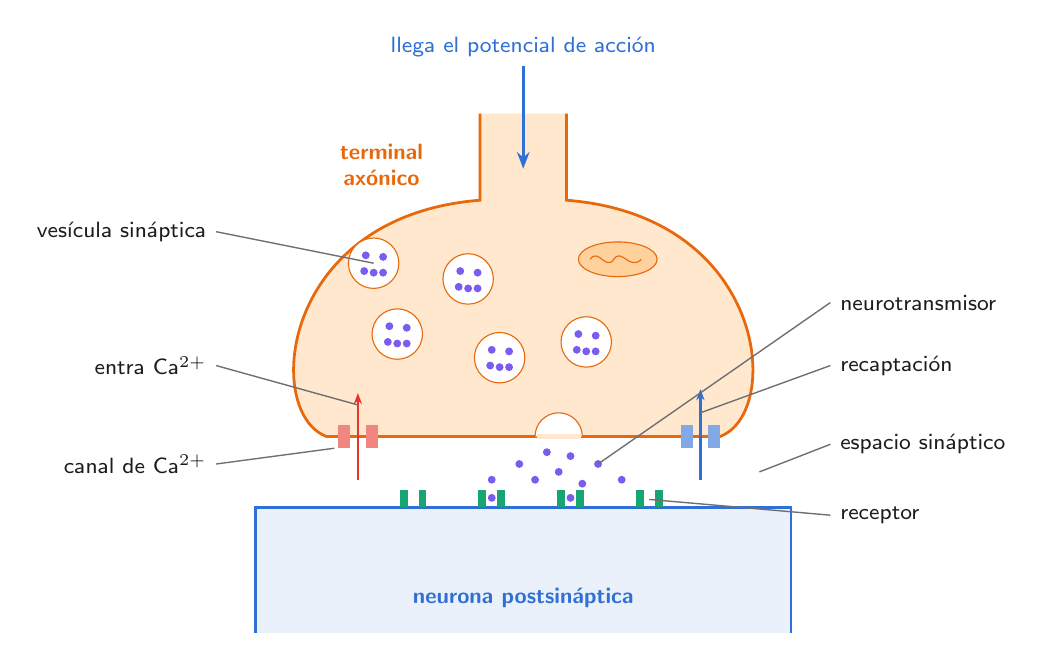
\begin{tikzpicture}[font=\footnotesize]
\sinapsis
\node[anchor=south,text=azul] at (0,6.0) {llega el potencial de acción};
\node[text=nar,font=\footnotesize\bfseries,align=center] at (-1.8,4.75) {terminal\\axónico};
\node[text=azul,font=\footnotesize\bfseries] at (0,-0.75) {neurona postsináptica};
\begin{scope}[gris,line width=0.5pt]
\draw (-1.9,3.5) -- (-3.9,3.9) node[anchor=east,text=tinta] {vesícula sináptica};
\draw (-2.1,1.7) -- (-3.9,2.2) node[anchor=east,text=tinta] {entra Ca$^{2+}$};
\draw (-2.4,1.15) -- (-3.9,0.95) node[anchor=east,text=tinta,align=right] {canal de Ca$^{2+}$};
\draw (0.95,0.95) -- (3.9,3.0) node[anchor=west,text=tinta] {neurotransmisor};
\draw (2.25,1.6) -- (3.9,2.2) node[anchor=west,text=tinta] {recaptación};
\draw (3.0,0.85) -- (3.9,1.2) node[anchor=west,text=tinta] {espacio sináptico};
\draw (1.6,0.5) -- (3.9,0.3) node[anchor=west,text=tinta] {receptor};
\end{scope}
\end{tikzpicture}
\end{document}
